不同编程语言的执行模型也不同,最常见的便是解释语言和编译语言。编译器将源代码翻译成机器代码,计算机可以在没有中间系统支持的环境下运行。另外,解释性语言代码需要支持系统、解释器和虚拟环境才能工作。 \par
C++是编译语言,所以会比解释型程序运行得更快。但C++程序需要针对每个平台进行编译,但解释型程序可以跨平台运行。 \par
我们将讨论程序构建的细节,从源代码阶段开始——由编译器完成——到可执行文件(编译器的输出)结束。还会去了解,为什么为一个平台构建的程序不能在另一个平台上运行。 \par
本章将讨论以下主题: \par

\begin{itemize}
	\item 介绍C++20。
	\item C++预处理的细节。
	\item 源代码的(底层)编译。
	\item 了解连接器及其功能。
	\item 加载和运行可执行文件的过程。
\end{itemize}

\noindent\textbf{}\ \par
\textbf{技术要求} \\
g++编译器需要添加编译选项 \texttt{-std=c++2a} 来编译本章的代码。可以从这里获取本章的源码文件:https:/​/github.​com/PacktPublishing/Expert-CPP \par

\noindent\textbf{}\ \par
\textbf{介绍C++20} \\
C++经过多年的发展,目前发展到C++ 20。自C++ 11以来,C++标准已经对语言的特性集进行了极大地扩展。现在,让我们来看看C++ 20标准中哪些值得关注的特性。 \par

\noindent\textbf{}\ \par
\textbf{概念(Concepts):}\ \par
概念是C++ 20的主要特性之一,它为类型提供了一组需求。概念的基本思想是模板参数的编译时进行验证,例如:要指定模板实参必须有默认构造函数,可以使用\textbf{default\underline{ }constructible}概念,方法如下: \par
\noindent\textbf{}\ \par

	%template <\textbf{default\underline{ }constructible} T> \par
	%void make\underline{ }T() { return T(); } \par
	
\begin{lstlisting}[caption={}]
template <default_constructible T>
void make_T() { return T(); }
\end{lstlisting}
	
\noindent\textbf{}\ \par
上面的代码中,我们忽略了typename关键字,设置一个概念来描述模板函数的形参T。\par

可以说概念是描述其他类型的类型——可称为元类型。允许在编译时验证模板参数,以及基于类型属性的函数调用。我们将在第3章和第4章中详细讨论这些概念。 \par

\noindent\textbf{}\ \par
\textbf{协程(Coroutines):}\ \par
协程是能够在执行点停止,并在稍后恢复的特殊函数。协程用以下关键字进行扩展:\par

\begin{enumerate}
	\item \texttt{co\underline{ }await} 暂停协程的执行。
	\item \texttt{co\underline{ }yield} 暂停协程的执行,同时返回一个值。
	\item \texttt{co\underline{ }return} 类似于return,完成协程时返回一个值。举个栗子:
\end{enumerate}

%	generator<int> step\underline{ }by\underline{ }step(int n = 0) \{ \par
%		\quad while (true) \{ \par
%			\quad \quad \textbf{co\underline{ }yield} n++; \par
%		\quad \} \par
%	\} \par

\begin{lstlisting}[caption={}]
generator<int> step_by_step(int n = 0) {
	while (true) {
		co_yield n++;
	}
}
\end{lstlisting}

\noindent\textbf{}\ \par
协程与promise对象相关联,promise可以存储协程的状态并发出警报。我们将在第8章中更深入地研究协程。 \par
	
\noindent\textbf{}\ \par
\textbf{范围(Ranges):}\ \par
范围库提供了一种处理元素范围的新方法。要使用它们,首先要包含<ranges>头文件。来看一个例子,范围是一个有开始和结束的元素vector,提供了一个begin迭代器和一个end哨兵:\par

\begin{lstlisting}[caption={}]
import <vector>
int main()
{
	std::vector<int> elements{0, 1, 2, 3, 4, 5, 6};
}
\end{lstlisting}

带有范围适配器(\texttt{|}操作符)的范围支持处理一系列元素的功能。看下代码: \par

\begin{lstlisting}[caption={}]
import <vector>
import <ranges>
int main()
{
	std::vector<int> elements{0, 1, 2, 3, 4, 5, 6};
	for (int current : elements | ranges::view::filter([](int e) { return
		e % 2 == 0; }))
	{
		std::cout << current << " ";
	}
}
\end{lstlisting}

前面的代码中,使用\texttt{ranges::view::filter()}过滤偶数。请注意\texttt{|}可以在不同的vector间使用。我们将在第7章中讨论范围及其强大的特性。 \par

\noindent\textbf{}\ \par
\textbf{更多C++20的特性}\ \par
C++ 20是一个大版本,它包含了许多更加复杂和灵活的特性。概念、范围和协程是本书讨论的众多特性中部分。 \par
最受期待的特性(之一)是模块,它提供了声明模块,以及在这些模块中导出类型和值的能力。可以将模块视为带有包含保护头文件,也就是头文件的改进版本。本章将介绍C++20中模块的特性。 \par
除了C++ 20中添加的一些特性外,我们还将在本书中讨论其他一些特性: \par

\begin{itemize}
	\item 超级操作符: \texttt{operator<=>()}。 现在可以利用\texttt{<=>()}来控制操作符重载的冗长程度。
	\item \texttt{constexpr}在这门语言中越来越常见。C++ 20现在添加了\texttt{consteval}函数、\texttt{constexpr std::vector}和\texttt{std::string}等类型。
	\item 数学常量,如\texttt{std::number::pi}和\texttt{std::number::log2e}。
	\item 线程库的更新,包括停止令牌和加入线程。
	\item 概念迭代器。
	\item 仅移动视图和其他功能。
\end{itemize}

为了更好地理解一些新特性并深入到该语言的本质,我们将从以前的版本开始介绍该语言的核心。这将有助于我们找到新特性相对于旧特性的更好用法,也将有助于支持历史遗留的C++代码。现在让我们从理解C++应用程序的构建开始。 \par

\noindent\textbf{}\ \par
\textbf{构建并运行程序}\ \par
可以使用任何文本编辑器来编写代码,因为代码就是文本。可以在简单的文本编辑器(如Vim)和高级集成开发环境(IDE)(如MS Visual Studio)之间自由选择。情书和源代码的唯一区别是后者可能由一种称为编译器的特殊程序解释(虽然情书不能被编译成程序,但它可能会让你紧张不安)。\par
为了区分文本文件和源代码,使用文件扩展名对二者进行区分。C++源码文件扩展为.cpp和.h(可能偶尔也会遇到.cxx和.hpp)。在讨论细节之前,请将编译器视为一种将源代码转换为可运行程序(即可执行文件)的工具,而源代码生成可执行文件的过程称为编译。编译C++程序是生成机器码的一系列复杂任务,机器码是计算机可以看得懂的语言。 \par
通常,C++编译器会解析和分析源码,然后生成中间码,对其进行优化,最后在目标文件中生成机器码。读者们可能见过目标文件了,它们有各自的扩展名,Linux中的.o和Windows中的.obj。所创建的目标文件不仅包含计算机可以运行的机器码,编译通常涉及几个源文件,编译每个源文件会生成一个目标文件。然后,这些目标文件通过链接器链接在一起,形成一个的可执行文件。链接器使用存储在目标文件中的附加信息,来正确地链接它们(链接将在本章后面讨论)。 \par
下面的图表描述了程序构建各个阶段: \par

\begin{center}
	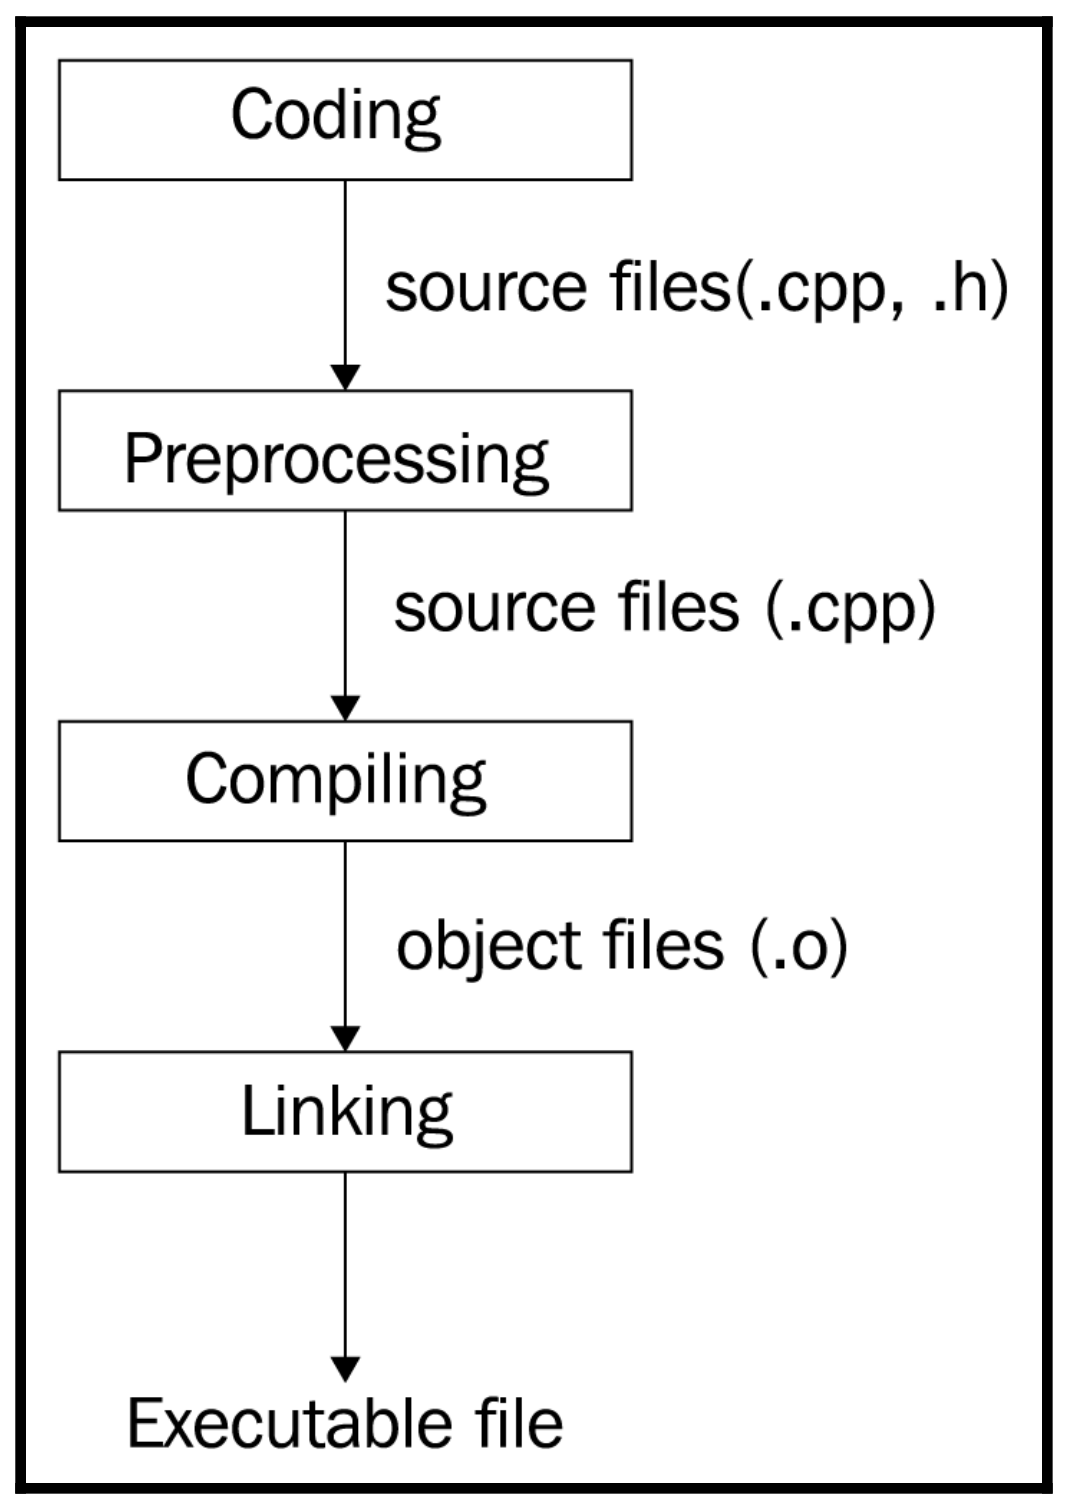
\includegraphics[width=0.3\textwidth]{content/Section-1/Chapter-1/1}
\end{center}

C++应用程序构建过程包括三个主要步骤:预处理、编译和链接。这些步骤使用不同的工具完成,但是编译器将它们封装在一个工具中,从而为程序员提供了更直接的接口。\par
生成的可执行文件保存在计算机的硬盘驱动器上,运行时会复制到主存RAM中,复制是由另一个名为加载器的工具完成。加载器是操作系统的一部分,它知道应该从可执行文件的内容中复制什么内容,以及在哪里复制。并且,加载的可执行文件不会从硬盘上删除。 \par
程序的加载和运行由操作系统(OS)完成,操作系统管理程序的执行,先执行优先级高的程序,完成后卸载程序等工作。程序的运行副本称为进程,进程是可执行文件的实例。 \par

\noindent\textbf{}\ \par
\textbf{预处理}\ \par
预处理器对源文件进行处理,使它们为编译做好准备。预处理器使用预处理器指令,比如\#define、\#include等等。指令不代表程序语句,但它们是预处理命令,告诉预处理器如何处理源文件的文本。编译器无法识别这些指令,因此无论何时在代码中使用预处理器指令,预处理器都会在代码开始实际编译之前解析它们。例如,以下代码将在编译器开始编译之前修改:\par

\begin{lstlisting}[caption={}]
#define NUMBER 41
int main() {
	int a = NUMBER + 1;
	return 0;
}
\end{lstlisting}

使用\#define指令是的定义称为宏。经过预处理后,编译器得到转换后的源文件如下: \par

\begin{lstlisting}[caption={}]
int main() {
	int a = 41 + 1;
	return 0;
}
\end{lstlisting}

预处理程序只处理文本,不关心语言规则或语法。使用预处理器指令,特别是宏定义,如前面的例子中,\#define NUMBER 41很容易出错,除非预处理器只是简单地将NUMBER替换为41,而没有将41解释为整数。对于预处理器,以下两行都是有效的:\par

\begin{lstlisting}[caption={}]
int b = NUMBER + 1;
struct T {}; // user-defined type
T t = NUMBER; // preprocessed successfully, but compile error
\end{lstlisting}

预处理后的代码: \par

\begin{lstlisting}[caption={}]
int b = 41 + 1
struct T {};
T t = 41; // error line
\end{lstlisting}

编译器开始编译时,发现t = 41是错误的,因为没有从'int'到' T'的转换。\par
使用语法正确,但有逻辑错误的宏非常危险: \par

\begin{lstlisting}[caption={}]
#define DOUBLE_IT(arg) (arg * arg)
\end{lstlisting}

预处理器将用(arg * arg)替换任何出现的DOUBLE\underline{}IT(arg),因此下面的代码将输出16: \par

\begin{lstlisting}[caption={}]
int st = DOUBLE_IT(4);
std::cout << st;
\end{lstlisting}

编译器接收到的代码如下所示: \par

\begin{lstlisting}[caption={}]
int st = (4 * 4);
std::cout << st;
\end{lstlisting}

当使用复杂表达式作为宏的参数时,会出现问题: \par

\begin{lstlisting}[caption={}]
int bad_result = DOUBLE_IT(4 + 1);
std::cout << bad_result;
\end{lstlisting}

这段代码期望输出25,但预处理程序除了文本处理之外什么都不做,所以会像这样替换宏:\par

\begin{lstlisting}[caption={}]
int bad_result = (4 + 1 * 4 + 1);
std::cout << bad_result;
\end{lstlisting}

输出是 9 ,而不是期望的25。 \par
对宏定义进行修正,需要在宏参数周围加上括号:\par

\begin{lstlisting}[caption={}]
#define DOUBLE_IT(arg) ((arg) * (arg))
\end{lstlisting}

现在预处理后的代码如下: \par

\begin{lstlisting}[caption={}]
int bad_result = ((4 + 1) * (4 + 1));
\end{lstlisting}

强烈建议在合适的情况下使用const声明,而非宏定义。 \par

\hspace*{\fill} \\ %插入空行

\includegraphics[width=0.05\textwidth]{images/tip}
经验法则:避免使用宏定义。宏易于出错,C++提供的构造方式可以不使用宏。 \par

\noindent\textbf{}\ \par
如果使用constexpr函数,则会在编译时检查类型并处理,使用上例: \par

\begin{lstlisting}[caption={}]
constexpr int double_it(int arg) { return arg * arg; }
int bad_result = double_it(4 + 1);
\end{lstlisting}

使用constexpr说明符可以在编译时计算函数的返回值(或变量的值)。有数字定义的例子最好使用const变量: \par

\begin{lstlisting}[caption={}]
const int NUMBER = 41;
\end{lstlisting}

\noindent\textbf{}\ \par
\textbf{头文件}\ \par
预处理器最常见的用法是\#include指令,用于在源代码中包含头文件。头文件包含函数、类等定义: \par

\begin{lstlisting}[caption={}]
// file: main.cpp
#include <iostream>
#include "rect.h"
int main() {
	Rect r(3.1, 4.05)
	std::cout << r.get_area() << std::endl;
}
\end{lstlisting}

假设头文件rect.h的定义如下: \par

\begin{lstlisting}[caption={}]
// file: rect.h
struct Rect
{
	private:
	double side1_;
	double side2_;
	public:
	Rect(double s1, double s2);
	const double get_area() const;
};
\end{lstlisting}

包含在rect.cpp中: \par

\begin{lstlisting}[caption={}]
// file: rect.cpp
#include "rect.h"
Rect::Rect(double s1, double s2)
: side1_(s1), side2_(s2)
{}
const double Rect::get_area() const {
	return side1_ * side2_;
}
\end{lstlisting}

预处理器检查main.cpp和rect.cpp之后,其会将\#include替换为相应的iostream头文件中的内容,并将rect.h的内容替换到main.cpp和rect.cpp中。C++17 引入了\underline{~~}has\underline{ }include 预处理常量表达式。 \underline{~~}has\underline{ }include如果找到指定名称的文件,则计算结果为1,否则为0: \par

\begin{lstlisting}[caption={}]
#if __has_include("custom_io_stream.h")
#include "custom_io_stream.h"
#else
#include <iostream>
#endif
\end{lstlisting}

声明头文件时,强烈建议使用包含保护(include-guards) (\#ifndef, \#define, \#endif)方式,以避免多重声明。同样,这些也是预处理器指令,以避免以下情况:\par

\begin{lstlisting}[caption={}]
// file: square.h
#include "rect.h"
struct Square : Rect {
	Square(double s);
};
\end{lstlisting}

在main.cpp中同时包含square.h和rect.h会导致包含rect.h两次: \par

\begin{lstlisting}[caption={}]
// file: main.cpp
#include <iostream>
#include "rect.h"
#include "square.h"
/*
	preprocessor replaces the following with the contents of square.h
*/
// code omitted for brevity
\end{lstlisting}

预处理后,编译器将接收到如下的main.cpp: \par

\begin{lstlisting}[caption={}]
// contents of the iostream file omitted for brevity
struct Rect {
	// code omitted for brevity
};
struct Rect {
	// code omitted for brevity
};
struct Square : Rect {
	// code omitted for brevity
};
int main() {
	// code omitted for brevity
}
\end{lstlisting}

然后,编译器将报出一个错误,因为它遇到了两个Rect类型的声明。头文件应该通过以下方式使用包含保护来防止多重包含: \par

\begin{lstlisting}[caption={}]
#ifndef RECT_H
#define RECT_H
struct Rect { ... }; // code omitted for brevity
#endif // RECT_H
\end{lstlisting}

当预处理器第一次遇到头文件时,RECT\underline{ }H没有定义,在\#ifndef和\#endif之间的语句都会进行处理,包括RECT\underline{ }H的定义。当预处理器第二次在同一源文件中包含同一头文件时,因为RECT\underline{ }H已经定义,所以会省略其中的内容。 \par
包含保护是控制源文件部分编译的指令的一部分。所有的条件编译指令为\#if、\#ifdef、\#ifndef、\#else、\#elif和\#endif。\par
条件编译在许多情况下非常有用,可以在调试模式下记录函数调用。在发布程序之前,建议对程序进行调试,并针对逻辑缺陷进行测试。你可能想看看调用某个函数后代码中会发生什么,例如: \par

\begin{lstlisting}[caption={}]
void foo() {
	log("foo() called");
	// do some useful job
}
void start() {
	log("start() called");
	foo();
	// do some useful job
}
\end{lstlisting}

每个函数会调用log()函数,其实现如下: \par

\begin{lstlisting}[caption={}]
void log(const std::string& msg) {
#if DEBUG
	std::cout << msg << std::endl;
#endif
}
\end{lstlisting}

如果定义了DEBUG, log()函数将打印msg。如果你编译的项目启用了DEBUG(使用编译器标记,例如\texttt{g++}中的\texttt{-D}),那么log()函数将打印传递给它的字符串,否则什么不做。 \par



























